%% Preamble %%
\documentclass[paper=a4]{article}

\usepackage{float}
\usepackage{geometry}
\geometry{verbose,tmargin=2.25cm,bmargin=2cm,lmargin=2.25cm,rmargin=2cm}
\geometry{a4paper}
\usepackage{multirow}


\usepackage[T1]{fontenc}
\usepackage{fourier}
\usepackage[utf8]{inputenc}
\usepackage[spanish]{babel}				

\usepackage{amsmath,amsfonts,amsthm} % Math packages
\usepackage[pdftex]{graphicx}	

\makeatletter
%%%%%%%%%%%%%%%%%%%%%%%%%%%%%% User specified LaTeX commands.
\usepackage{fancyhdr}
\usepackage{lscape}
\pagestyle{fancy}
\lhead{Electr\'onica II 22.12}
\chead{TPL1}
\rhead{ITBA}
\renewcommand{\headrulewidth}{1pt}
\renewcommand{\footrulewidth}{1pt}

\makeatother

\usepackage{babel}
\addto\shorthandsspanish{\spanishdeactivate{~<>}}

\begin{document}

\tableofcontents
\newpage

\section{Objetivos - Parámetros del sistema}

En el presente trabajo práctico se realiza el diseño e implementación de un amplificador de audio de un solo canal, con las siguientes especificaciones:

\begin{center}
\begin{tabular}{|c|c|}
\hline 
$P_{O_{MAX}}[W]$ & $Z_{IN}[\Omega]$\\
\hline 
\hline 
$22$ & $50K$\\
\hline 
\end{tabular}
\end{center}

La carga nominal para el diseño considerada es de $8\Omega$, y se trabajará en el rango de frecuencias de audio. Es decir, en la banda de 20Hz a 20KHz. La sensibilidad de la entrada a $P_{O_{MAX}}$ es de 1$V_{pp}$.

\section{Diseño del sistema}

El circuito propuesto es un amplificador con salida diferencial, utilizando etapas de potencia clase AB con simetría complementaria. El circuito simplificado se muestra a continuación.

\begin{figure}[!ht]
\begin{centering}
\includegraphics[scale=0.45]{Imagenes/CompletoSimple.png}
\par\end{centering}
\caption{Circuito amplificador con salida diferencial (simplificado)}
\end{figure}

Para tener un cierto margen a las especificaciones propuestas, se diseñará para una potencia de $25W$ sobre la carga.

\newpage

\subsection{Etapa de salida}

El circuito en cuestión es algo no tan común dado que la salida no está referida a masa, sino que la misma es diferencial. En la figura se muestra centralmente la etapa de salida para analizar.

\begin{figure}[!ht]
\begin{centering}
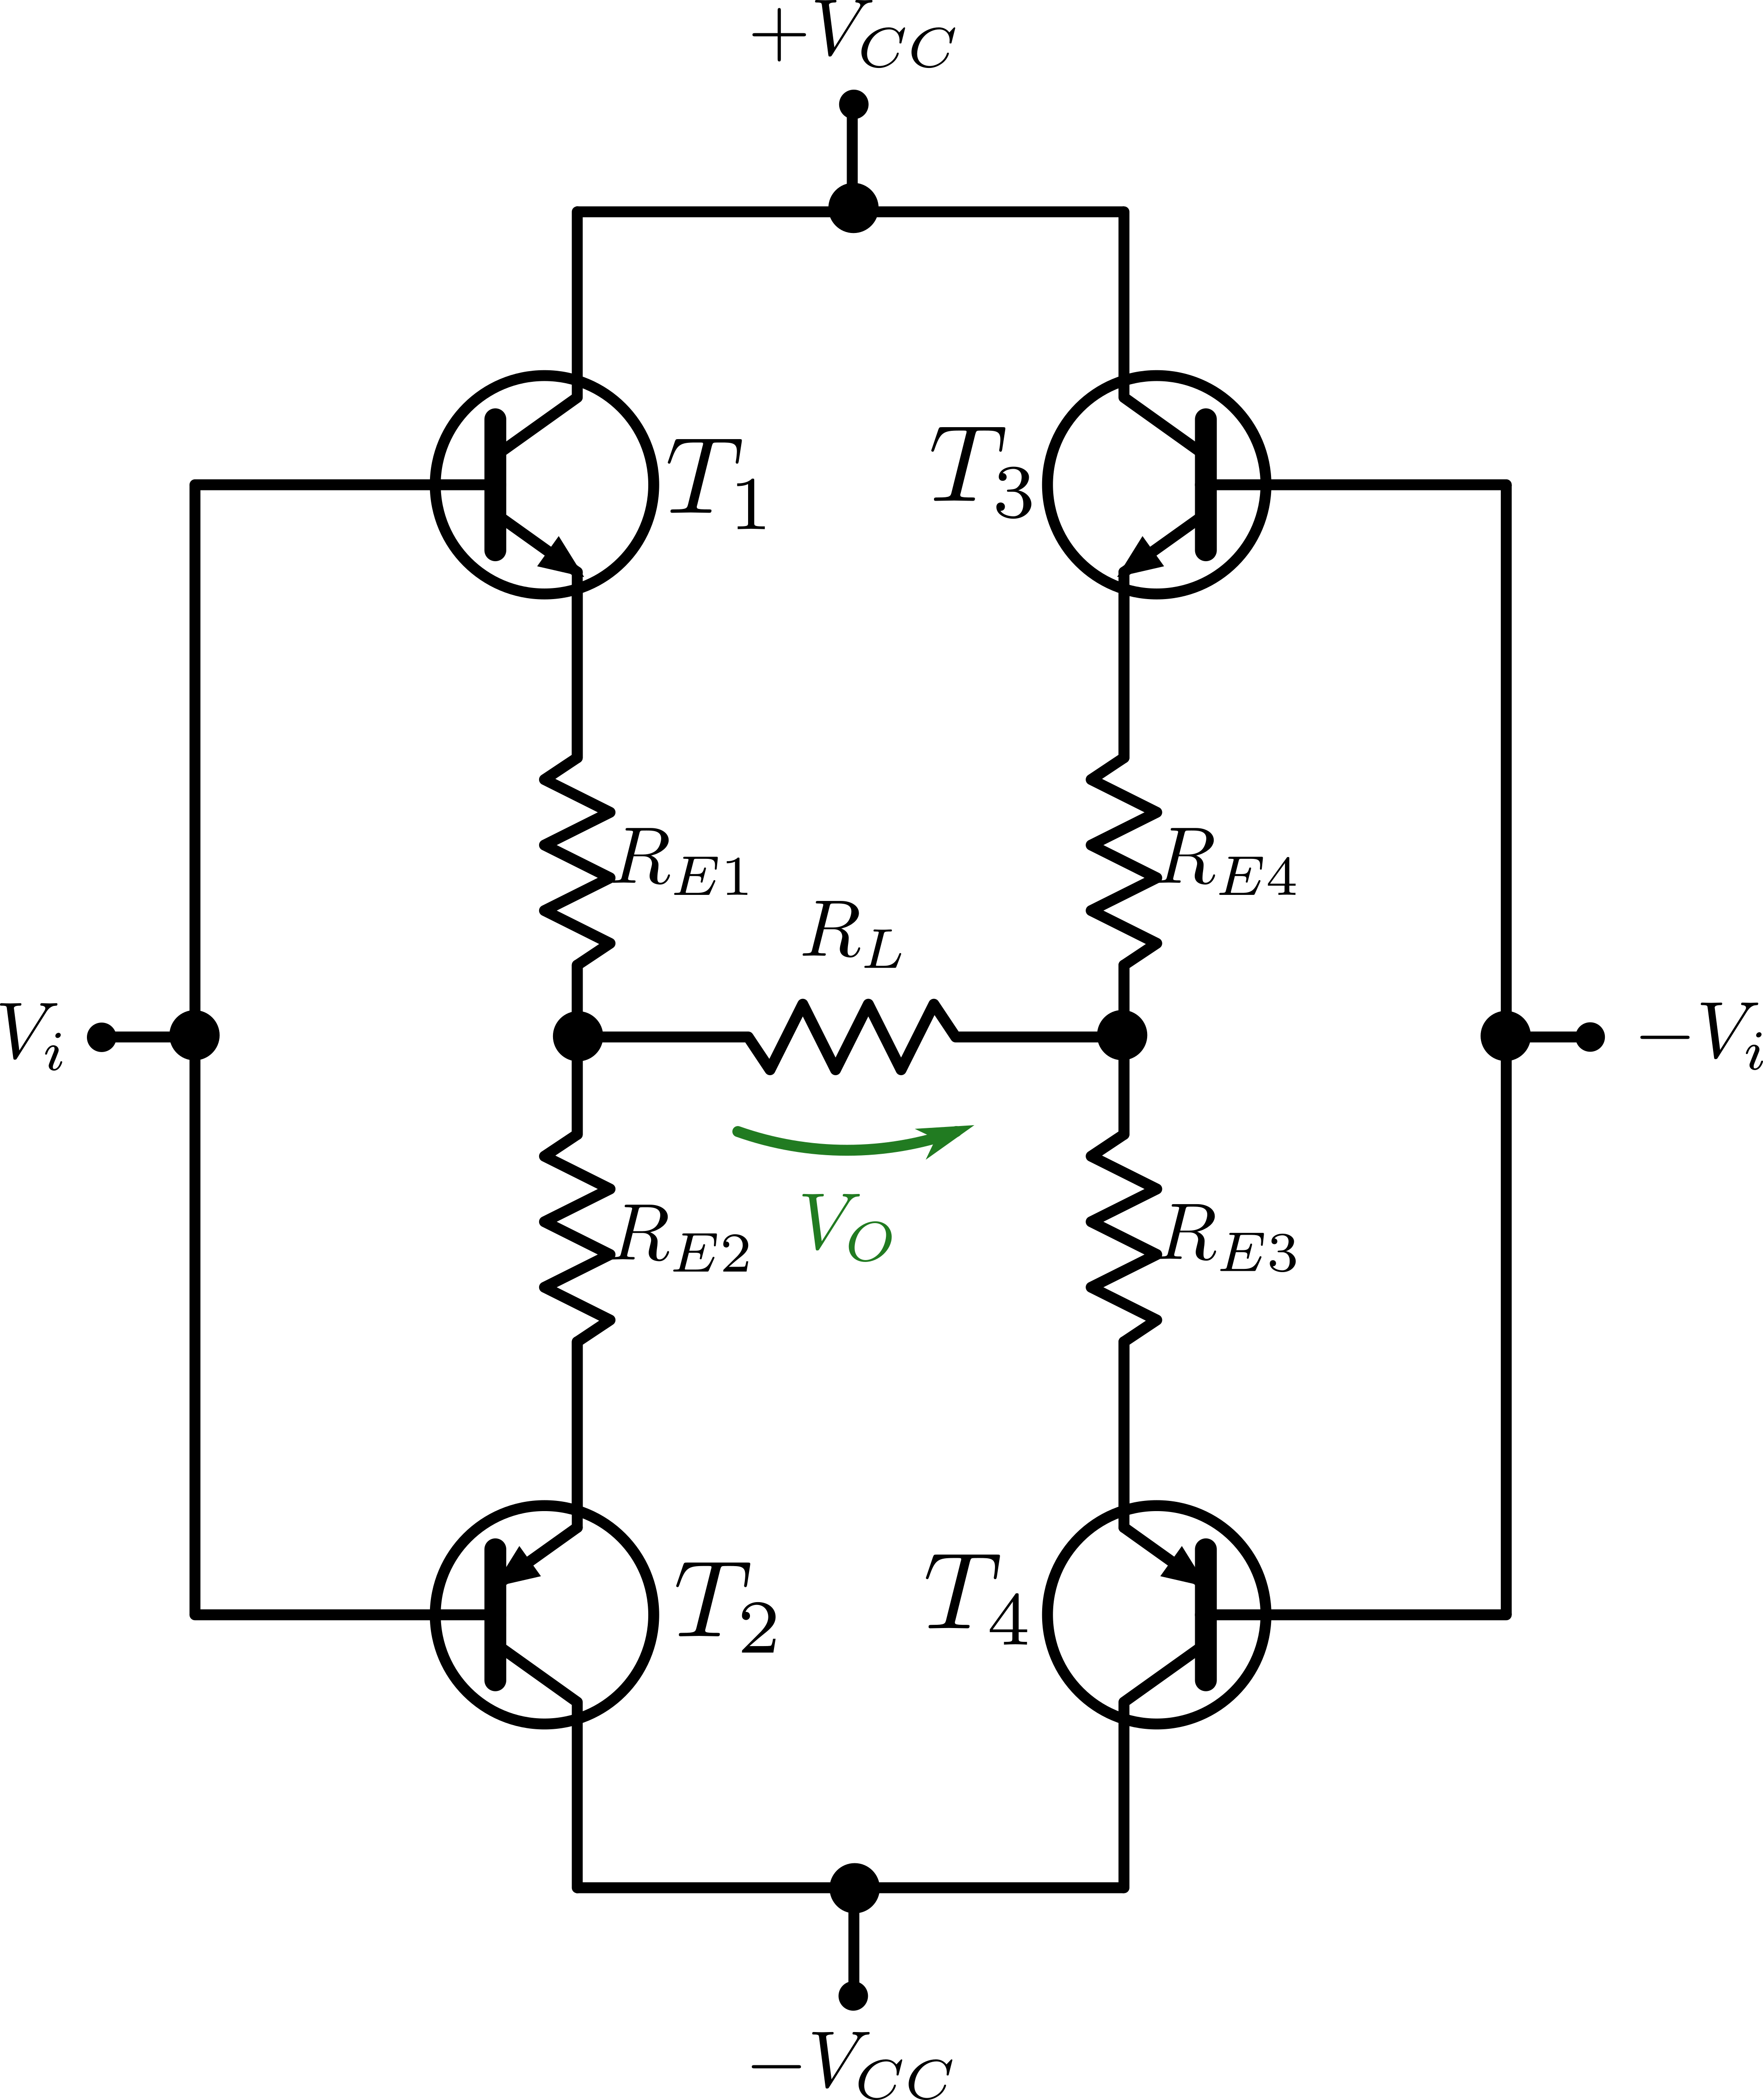
\includegraphics[scale=0.5]{Imagenes/EtapaSalida.png}
\par\end{centering}
\caption{Etapa de salida diferencial}
\end{figure}

Teniendo la potencia buscada sobre la carga, se puede realizar el diseño del amplificador desde ``afuera hacia adentro'' (es decir, desde la salida hacia el generador de entrada).\par
Siendo que se trabaja con señales senoidales, la potencia de salida que se toma en cuenta es la potencia eficaz, teniendo:

\[
P_{O_{MAX}} = \frac{V_{O_{RMS}}}{R_L} = \frac{{\hat{V_O}_{MAX}}^2}{2 \cdot R_L}
\]

Considerando para el diseño que $P_{O_{MAX}} = 25W$, se calcula la $\hat{V_O}_{MAX}$ necesaria:

\[
P_{O_{MAX}} = \frac{{\hat{V_O}_{MAX}}^2}{2 \cdot R_L} \Longrightarrow \hat{V_O}_{MAX} = \sqrt{2 \cdot R_L \cdot P_{O_{MAX}}} = 20V
\] 

Dicha tensión sería la tensión pico máxima diferencial sobre la carga. Tomando uno de sus bornes respecto de masa, es la mitad del valor, es decir $\frac{\hat{V_O}_{MAX}}{2} = 10V$.\par
Con la tensión calculada, se puede obtener la $\hat{I_O}_{MAX}$ sobre la carga:

\[
\hat{I_O}_{MAX} = \frac{\hat{V_O}_{MAX}}{R_L} = 2.5A
\]

Unos transistores de potencia adecuados a estas especificaciones son los darlington complementarios TIP122 (NPN) y TIP127 (PNP). Por lo que se seleccionan $T_1 = T_3 = \textrm{TIP122}$ y $T_2 = T_4 = \textrm{TIP127}$.\par
Las resistencias $R_{E1}$, $R_{E2}$ $R_{E3}$ y $R_{E4}$ se colocan para evitar que los transistores se quemen debido al efecto que se conoce como ``embalamiento térmico''. Esto se explica más en detalle junto con el efecto de distorsión por cruce por cero en la sección sobre prepolariación.

%FALTA REVISAR LA EXPLIACION ESTA!!!

Esta implementación presenta algunas ventajas respecto de una con salida referida a masa. En el caso de este último (correspondería tomar solo una de las dos mitades del circuito), cada fuente de alimentación aporta corriente en uno de los dos semiciclos de señal (dado que en cada semiciclo conduce solo uno de los dos transistores NPN o PNP), mientras que en la implementación propuesta ambas fuentes proporcionan corriente en ambos semiciclos. En el semiciclo positivo (es decir, tomando $V_i > 0$) conducen los transistores $T_1$ y $T_4$, mientras que en el negativo conducen $T_2$ y $T_3$. Esta configuración es conocida como ``Puente H'', la cual es común implementarla en el control de sentido de giro de un motor (siendo el motor la carga $R_L$).\par
Se considera nuevamente:

\[
P_{O_{MAX}} = \frac{{\hat{V_O}_{MAX}}^2}{2 \cdot R_L}
\]

Para observar una de las ventajas de esta implementación, se toma medio circuito (como se mencionó anteriormente), diseñándolo para una cierta potencia $P_{O_{MAX}}$, que dará lugar a una $\hat{V_O}_{MAX}$. El otro hemicircuito será similar pero con una fase de $180^{\circ}$. Conectando la carga $R_L$ entre ambas salidas, en cada terminal de la misma se tendría entonces $V_O$ y $-V_O$ respectivamente. Esto quiere decir que sobre la carga se tendría una diferencia de tensión de $2V_O$. Si se reemplaza en la ecuación de potencia anterior, resulta que la $P_{O_{MAX}}$ en el circuito propuesto es cuatro veces mayor que para el mismo diseño sobre un circuito con salida referida a masa, utilizando fuentes de alimentación de igual valor de tensión en ambos casos (pero las fuentes deberán ser del doble de potencia para el circuito diferencial).\par
Se detalla el cálculo de las potencias en la sección de cálculo de protección térmica con disipador.

\subsection{Prepolarización}

En la etapa de salida clase B mostrada previamente, surge el inconveniente de que, cuando la señal de control a sus bases es menor a la $V_{BE_{ON}}$ correspondiente, ninguno de los transistores conduce, por lo que durante ese intervalo de tiempo la tensión sobre la carga es nula.\par
Este efecto se conoce como distorsión de ``cruce por cero''. Para reducir dicho efecto, se busca darle a los transistores una tensión sobre la base para prepolarizarlos. Una manera efectiva de implementar esto es mediante el circuito conocido como multiplicador de $V_{BE}$, que se muestra a continuación.

\begin{figure}[!ht]
\begin{centering}
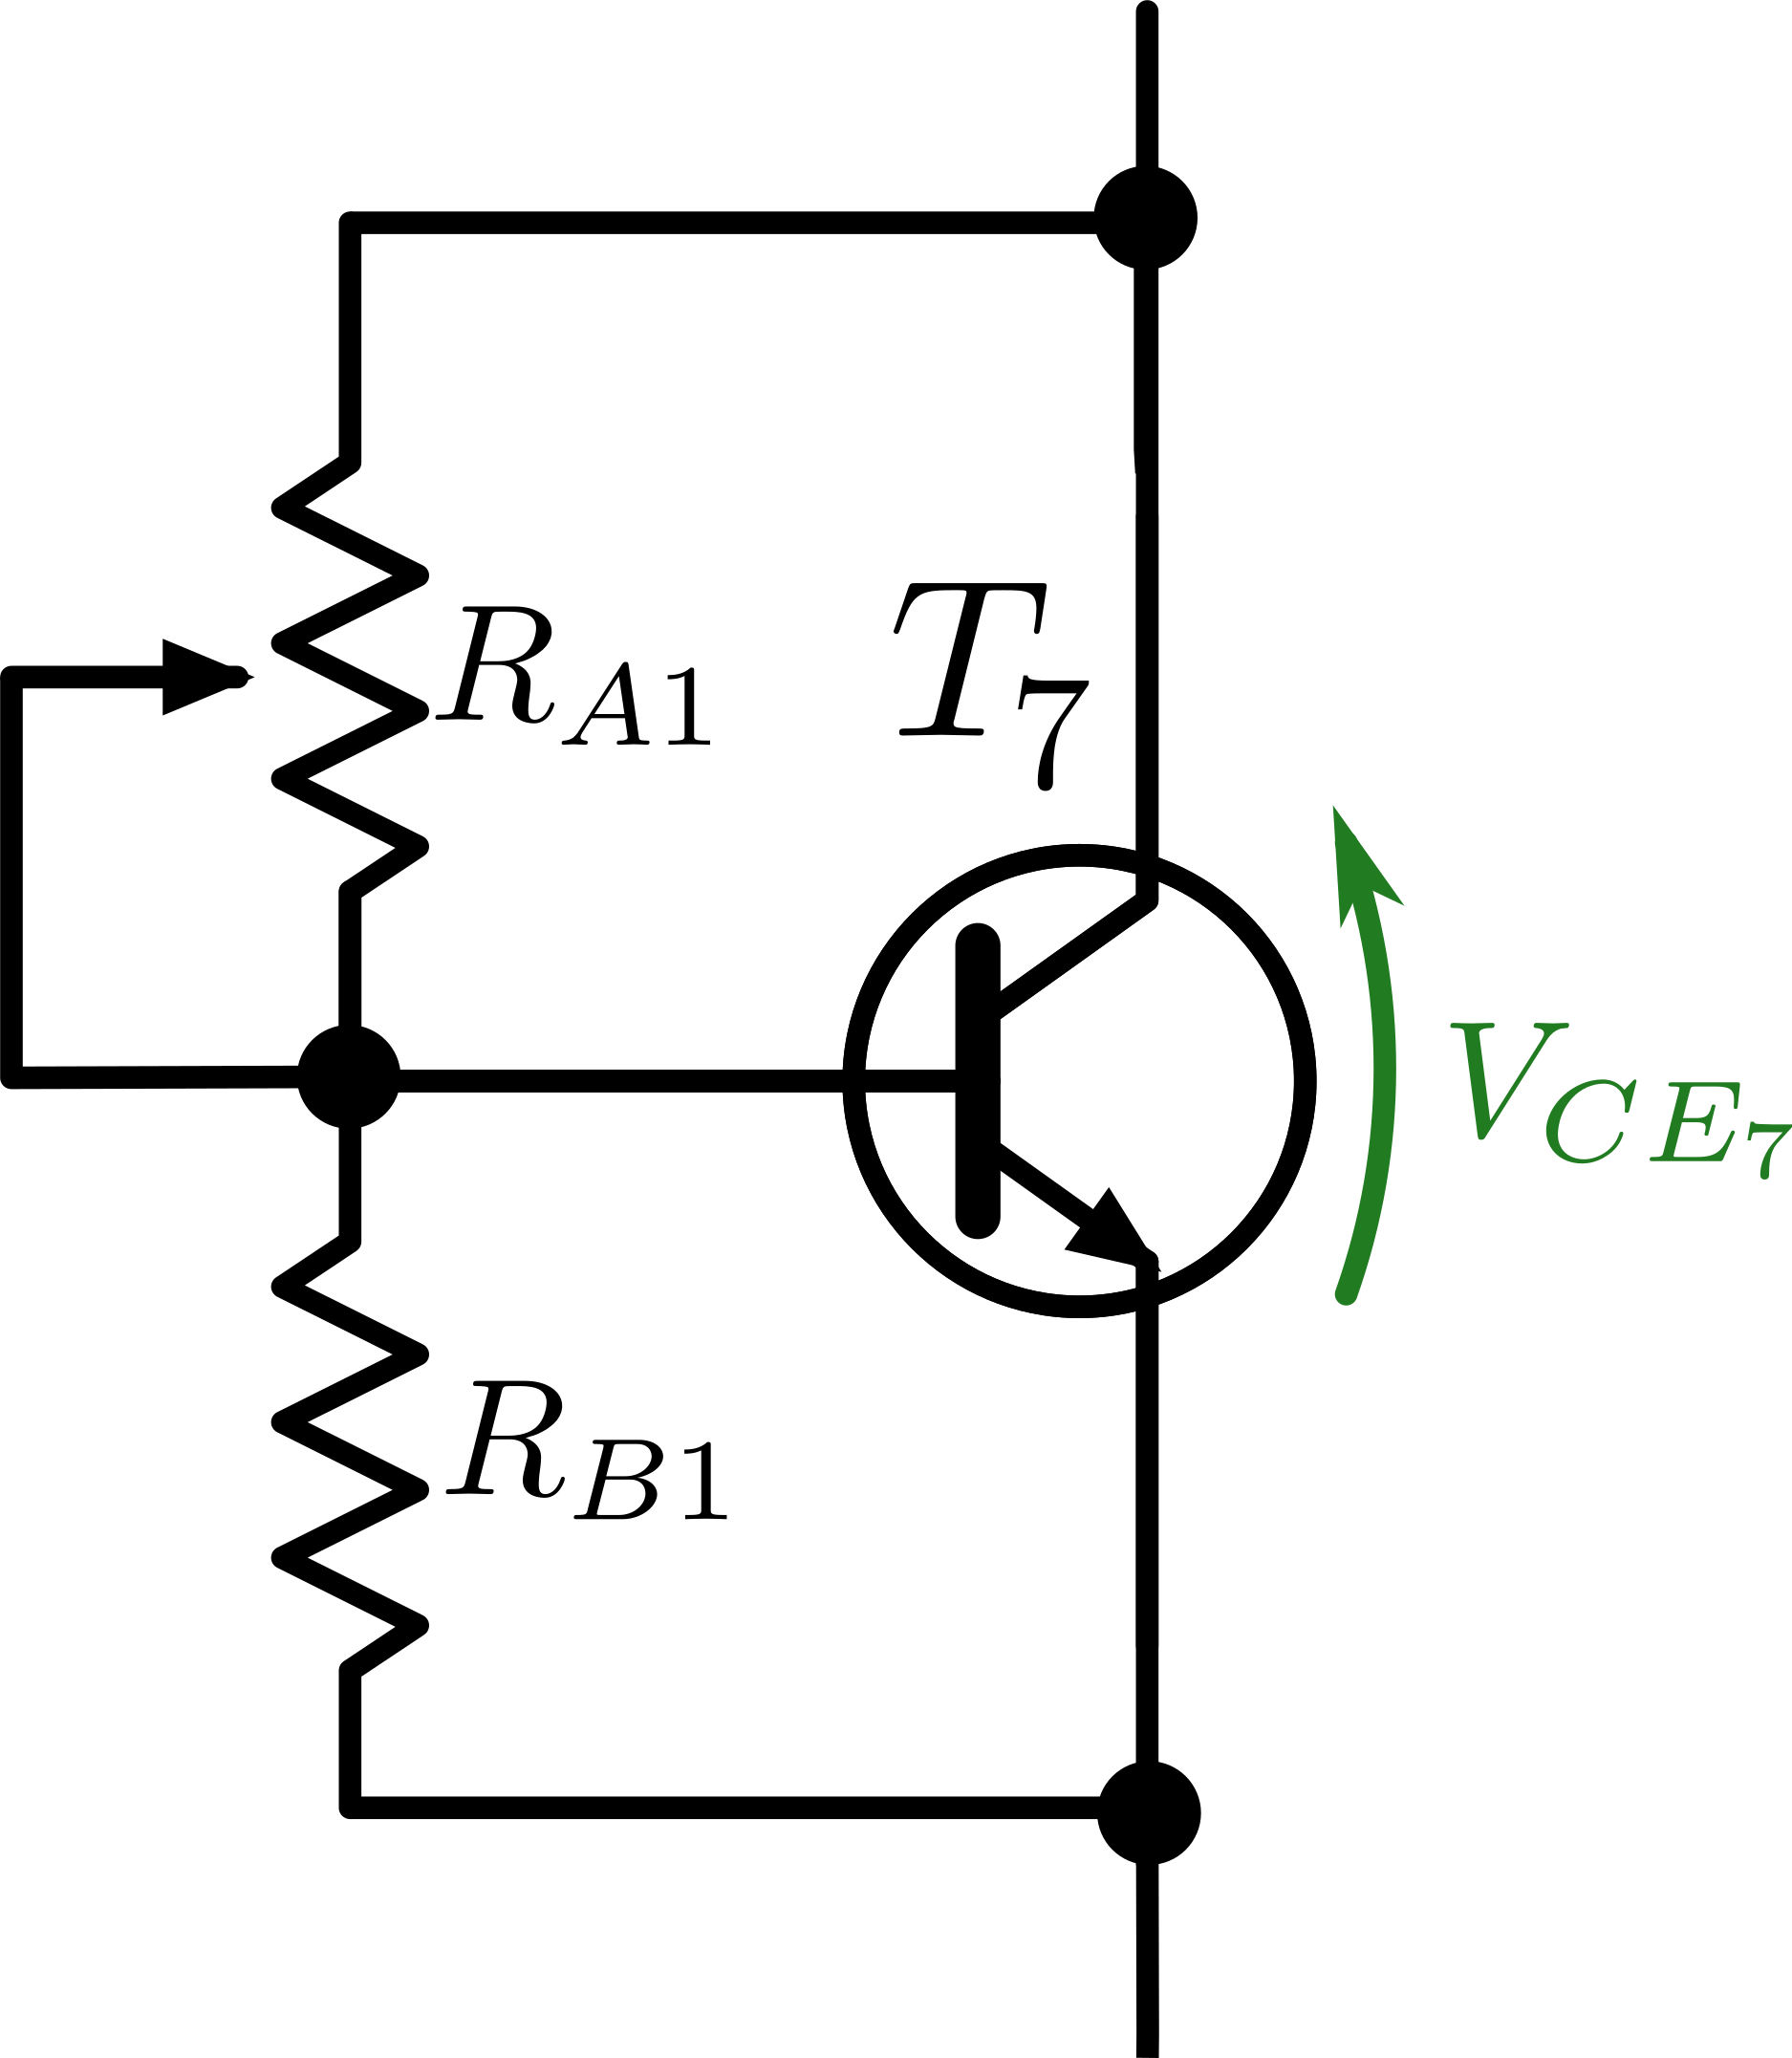
\includegraphics[scale=0.5]{Imagenes/MultiplicadorVBE.png}
\par\end{centering}
\caption{Multiplicador de $V_{BE}$}
\end{figure}

El colector y el emisor del transistor $T_7$ se conectan a las bases de los transistores de potencia respectivamente. En el hemicircuito izquierdo corresponde a $T_1$ y $T_2$, y para el hemicircuito derecho corresponde a $T_3$ y $T_4$ (al igual que la fuente de corriente $I_F$, se utliza un multiplicador de $V_{BE}$ por cada hemicircuito con idénticos componentes).\par
Planteando el divisor resistivo sobre $V_{BE7}$:

\[
V_{BE7} = V_{CE7} \cdot \left( \frac{R_{B1}}{R_{A1} + R_{B1}} \right)
\]

Despejando $V_{CE7}$ resulta:

\[
V_{CE7} = V_{BE7} \cdot \left( 1 + \frac{R_{A1}}{R_{B1}} \right)
\]

Para prepolarizar cada transistor del hemicircuito, se necesita una $V_{BE_{ON}} = 1.4V$ en cada uno, lo que resulta un total de 2.8V. Si se utiliza $R_{A1} = 10K\Omega$ como preset para ajuste, se despeja $R_{B1}$:

\[
R_{B1} = \frac{R_{A1}}{\frac{2.8V}{0.7V} - 1} = 3.33K\Omega \Longrightarrow R_{B1}(N) = 2.7K\Omega
\]

Se normaliza hacia abajo para asegurar la tensión mínima buscada (ya que $R_{B1}$ divide en la fórmula).\par
Hay otro inconveniente en este tipo de etapas de salida. Suponiendo que las resistencias de emisor $R_E$ colocadas en el diseño final no estuvieran, consideremos el caso donde se entrega corriente alta a la carga. En este caso los transistores de salida elevarán su temperatura, debido a la potencia que disipan. Al elevar su temperatura, la curva $I_C(V_{BE})$ resulta ``desplazada'' hacia la izquierda, es decir que para la misma $V_{BE}$ resulta una $I_C$ mayor. Al aumentar un poco la $I_C$, la temperatura aumenta también dado que la potencia disipada en los transistores aumenta, desplazándose nuevamente la curva $I_C(V_{BE})$, repitiéndose el proceso hasta que los dispositivos se destruyen. Esto se conoce (como se mencionó anteriormente) como embalamiento térmico. Para evitar este efecto, se introducen las resistencias $R_E$ indicadas anteriormente en los emisores de los transistores, siendo de bajo valor (un criterio que se suele tomar es que resulten 10 veces menores al valor de la carga para evitar pérdidas de potencia significativas).\par
En base a los valores disponibles, se colocaron resistencias $R_{E1} = R_{E2} = R_{E3} = R_{E4} = 0.33\Omega$. Para saber de qué potencia deben ser para no quemarse, se calcula la potencia eficaz máxima que disiparán. Siendo la $\hat{I_O}_{MAX} = 2.5A$, se tiene:

\[
\left. P_{R_E} \right|_{I_O \textrm{es máxima}} = \frac{\hat{I_O}_{MAX}^2}{2} \cdot R_E = 1.1W
\]  

Se colocaron entonces las de potencia normalizada siguiente hacia arriba disponibles, que fueron las de 3W.

\subsection{Fuente de corriente $I_F$}

Para las fuentes de corriente $I_F$ expresadas en el diseño, se implementó el siguiente circuito:

\begin{figure}[!ht]
\begin{centering}
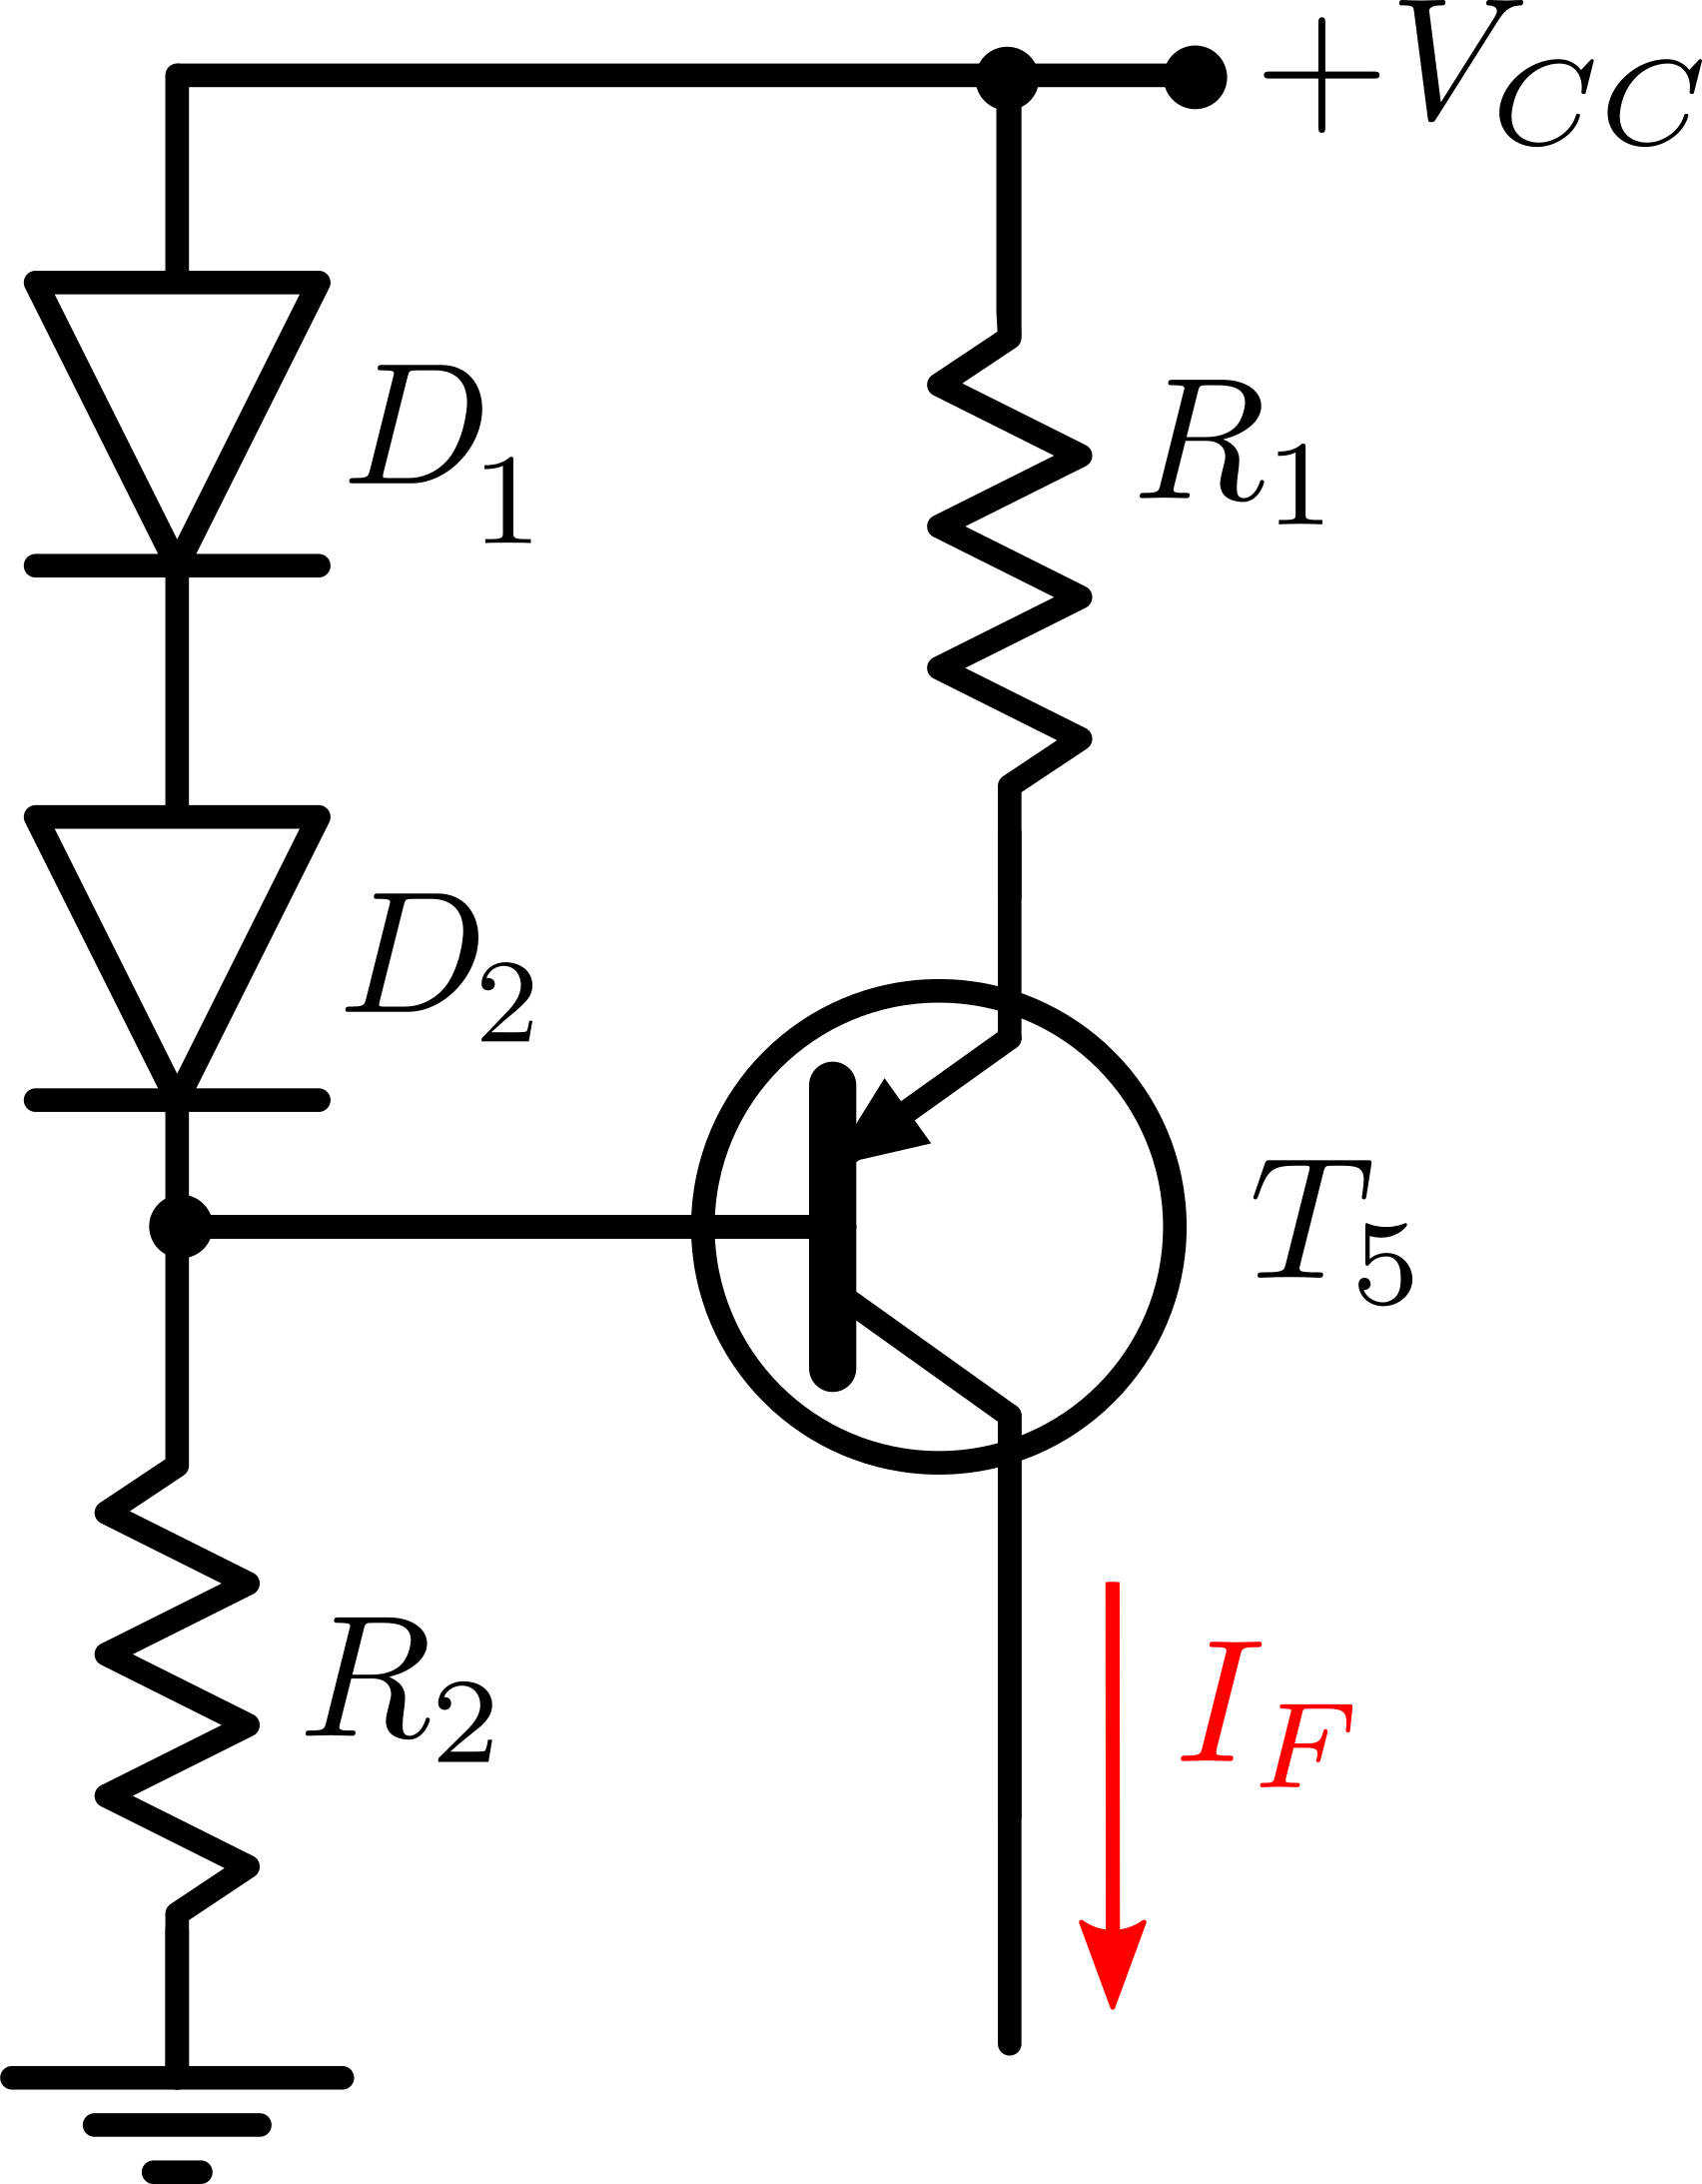
\includegraphics[scale=0.5]{Imagenes/FuenteIF.png}
\par\end{centering}
\caption{Fuente de corriente}
\end{figure}

Dado que la función de los diodos $D_1$ y $D_2$ es solamente provocar una caída de tensión similar a la $V_{EB5_{ON}}$, se utilizan los comunes 1N4148. Considerando que $R_2$ permite polarizarlos correctamente, se tiene recorriendo la malla:

\[
V_{D2} + V_{D1} - I_F \cdot R_1 - V_{EB5_{ON}} = 0
\]

Considerando $V_{D1} = V_{D2} = V_{EB5_{ON}} = V_D = 0.7V$, se tiene:

\[
I_F \cdot R_1 = V_D \Longrightarrow R_1 = \frac{V_D}{I_F}
\]

Del diseño de la etapa de potencia se obtuvo que $\hat{I_O}_{MAX} = 2.5A$. Considerando que los transistores TIP utilizados poseen un $HFE_{MIN} = 1000$ según la hoja de datos (ON Semiconductor), se calcula la corriente de base mínima necesaria que deberá poder proveerles la fuente de corriente (tomando de referencia al transistor $T_1$):

\[
\left. I_{B1_{MIN}} \right|_{I_{O_{MAX}}} = \frac{\hat{I_O}_{MAX}}{HFE_{MIN}} = 2.5mA \Longrightarrow I_{F_{MIN}} = 2.5mA
\]

Entonces se tiene:

\[
R_{1_{MAX}} = \frac{V_D}{I_{F_{MIN}}} = 280\Omega \Longrightarrow R_1(N) = 270\Omega
\]

Se normaliza hacia abajo para asegurar la $I_{F_{MIN}}$.\par
Teniendo ya la etapa de potencia y la fuente de corriente diseñadas, se puede determinar la $V_{CC_{MIN}}$ de acuerdo al camino formado desde la carga, pasando por $R_{E1}$, $T_1$ (como referencia tomando el semiciclo positivo), $T_5$ y $R_1$. Recordando que en un borne de la carga respecto a masa se tiene en el peor caso $\frac{\hat{V_O}_{MAX}}{2}$:

\[
\frac{\hat{V_O}_{MAX}}{2} + \hat{I_O}_{MAX} \cdot R_{E1} + V_{BE1_{ON}} + V_{EC5_{SAT}} + V_D = V_{CC_{MIN}} \Longrightarrow V_{CC_{MIN}} = 13.625V
\]

Como fuente normalizada se utilizará $V_{CC} = \pm 15V$, para asegurar dichas tensiones en el peor caso, considerando además que la tensión que entrega la fuente puede caer un pequeño porcentaje al trabajar con la carga a potencia máxima.\par
Con la fuente de tensión definida, se puede calcular ahora $R_2$ de manera de asegurar la polarización de los diodos. Tomando una corriente en directa $I_D$ para los diodos 1N4148 de 2mA, se tiene (despreciando la corriente de base de $T_5$):

\[
V_{CC} - 2 \cdot V_D - I_D \cdot R_2 = 0
\]

\[
 R_{2_{MAX}} = \frac{V_{CC} - 2 \cdot V_D}{I_D} = 6.8K\Omega \Longrightarrow R_2(N) = 4.7K\Omega
\]

Normalizando hacia abajo de manera tal de asegurar la $I_D$.\par
Dado que no hay requerimientos particulares de corriente o tensión sobre $T_5$, se utiliza de los disponibles el BC327.\par
Para la fuente de corriente del otro hemicircuito, los componentes son idénticos.

\subsection{Etapa de ganancia de tensión}

Para la etapa de ganancia de tensión, se utiliza un amplificador operacional en configuración no inversor. El integrado utilizado es el TL084, de los más comunes utilizados en audio, dada su baja distorsión armónica y alta impedancia de entrada. El circuito en cuestión es el siguiente.

\begin{figure}[!ht]
\begin{centering}
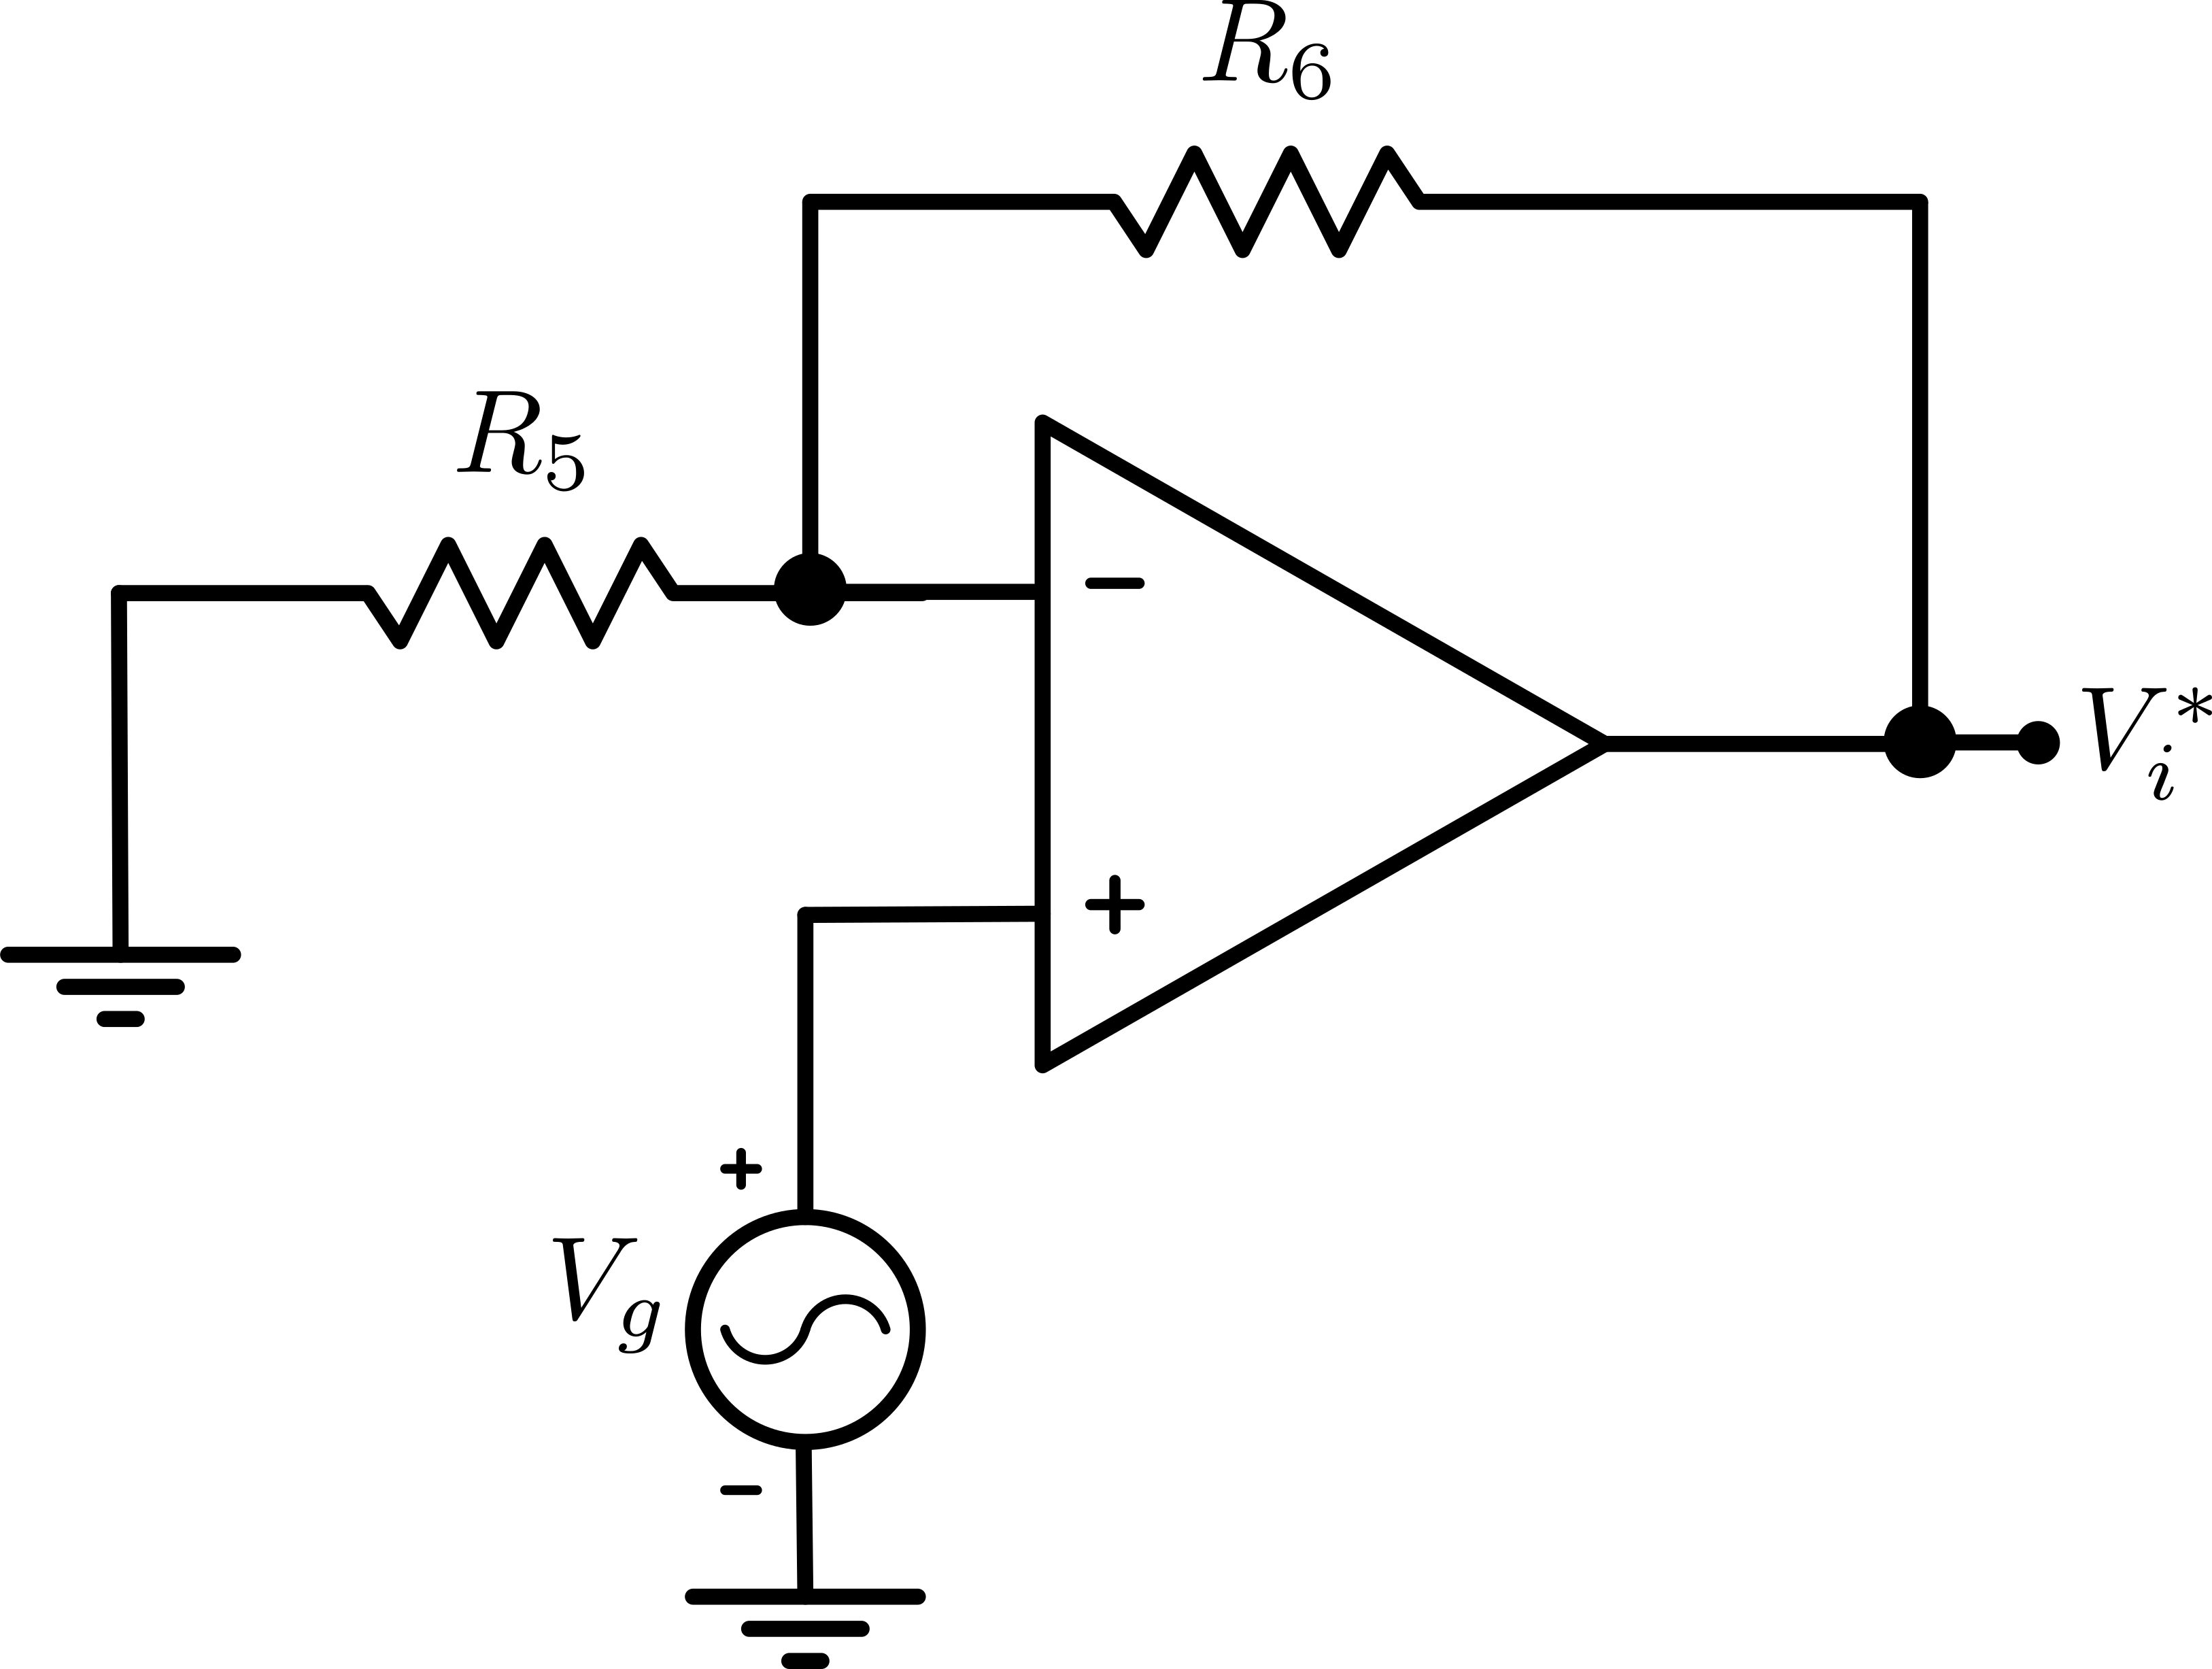
\includegraphics[scale=0.5]{Imagenes/EtapaDeAV.png}
\par\end{centering}
\caption{Amplificador de tensión}
\end{figure}

Dado que la etapa de salida es colector común, se aproxima su ganancia de tensión como unitaria por simplicidad. Sabiendo entonces que se da como parámetro que para la máxima potencia de salida, la señal de entrada es $\hat{V_g}_{MAX} = 0.5V$, y que en cualquiera de los bornes de la carga se tiene en dicho caso $\frac{\hat{V_O}_{MAX}}{2} = 10V$ respecto de masa, la ganancia de tensión necesaria es de:

\[
A_V = \frac{V_i^*}{V_g} = \frac{ \frac{\hat{V_O}_{MAX}}{2} }{\hat{V_g}_{MAX}} = 20
\]

De la expresión conocida para la ganancia de tensión del no inversor:

\[
A_V = \left( 1 + \frac{R_6}{R_5} \right) = 20
\]

Se toman $R_5(N) = 10K\Omega$, y $R_6(N) = 180K\Omega + 10K\Omega$ (serie).

Para producir la señal invertida para el otro hemicircuito, se toma la salida $V_i^*$ de esta etapa y se conecta a otro amplificador operacional en configuración inversora de ganancia de tensión -1. En la figura se muestra como queda dicho conjunto.

\begin{figure}[!ht]
\begin{centering}
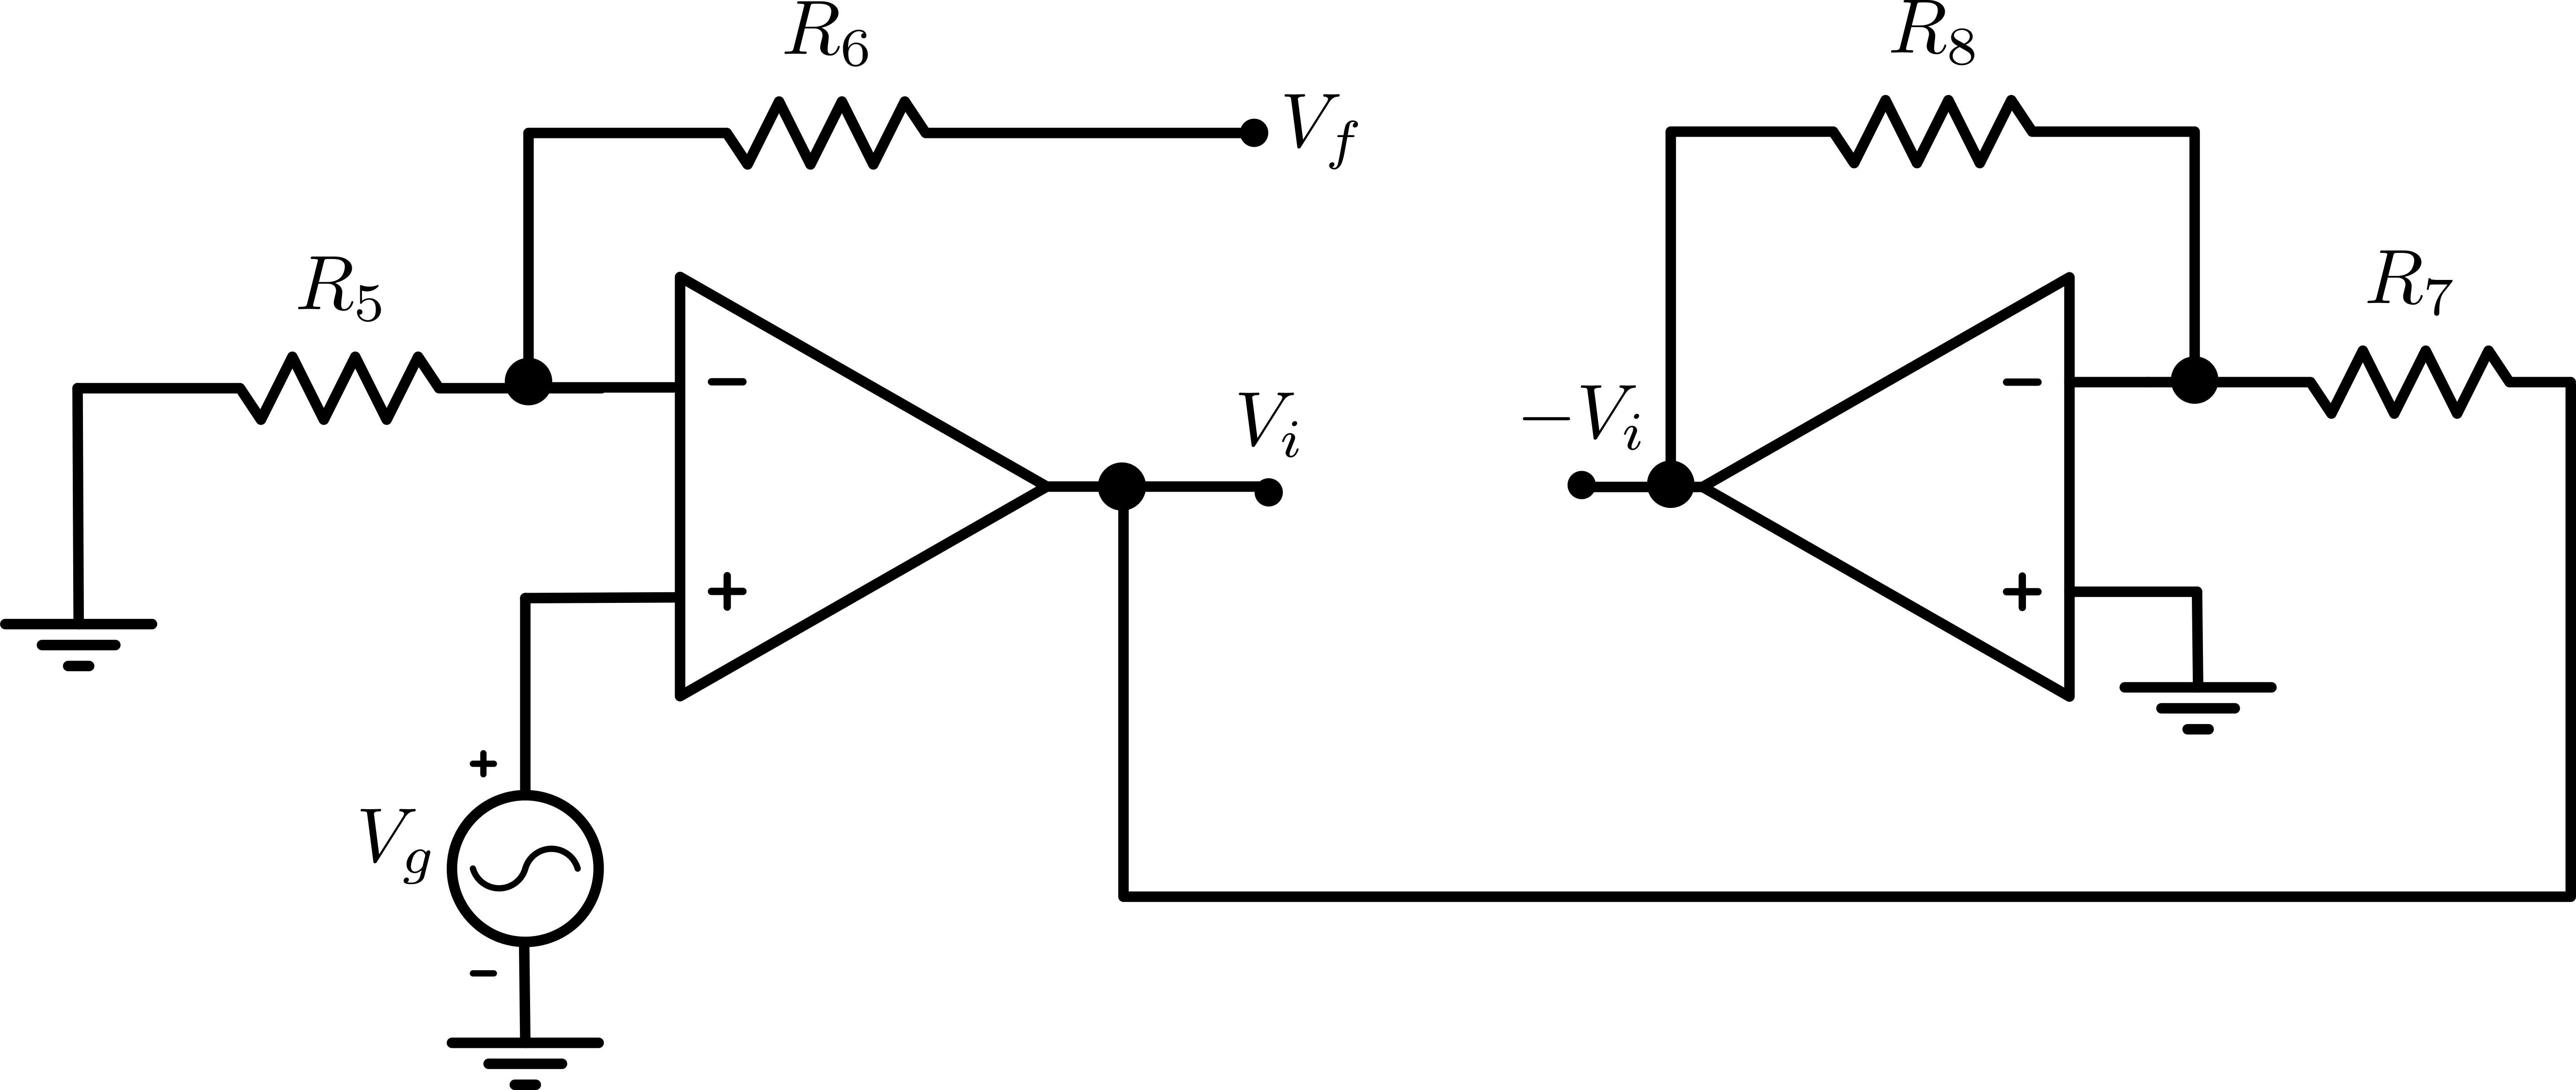
\includegraphics[scale=0.5]{Imagenes/opamp2SinCap.png}
\par\end{centering}
\caption{Amplificador de tensión e inversión de señal}
\end{figure}

Para obtener la ganancia del inversor $A_V = -1$, de la expresión conocida:

\[
A_V = -\frac{R_8}{R_7}
\]

Se toman por simplicidad $R_7(N) = R_8(N) = 10K\Omega$.
En la figura se hace una distinción particular con $V_f$, dado que la ganancia se calculó tomando como tensión que muestrea el lazo como $\frac{\hat{V_O}_{MAX}}{2}$. Como la señal a muestrear debe ser la salida del circuito y ésta es diferencial, se debe tomar dicha salida y hacer la diferencia propiamente dicha, dividida por 2. Es decir:

\[
V_f = \frac{1}{2}\left( \frac{\hat{V_O}_{MAX}}{2} - \left( -\frac{\hat{V_O}_{MAX}}{2} \right) \right) = \frac{\hat{V_O}_{MAX}}{2}
\]

De esta manera, la señal muestreada resultante $V_f$ es la llamada en el primer circuito como $V_i^*$. Para efectuar dicha operación, se implementa un tercer amplificador operaciónal en configuración de restador, como se muestra a continuación.

\begin{figure}[!ht]
\begin{centering}
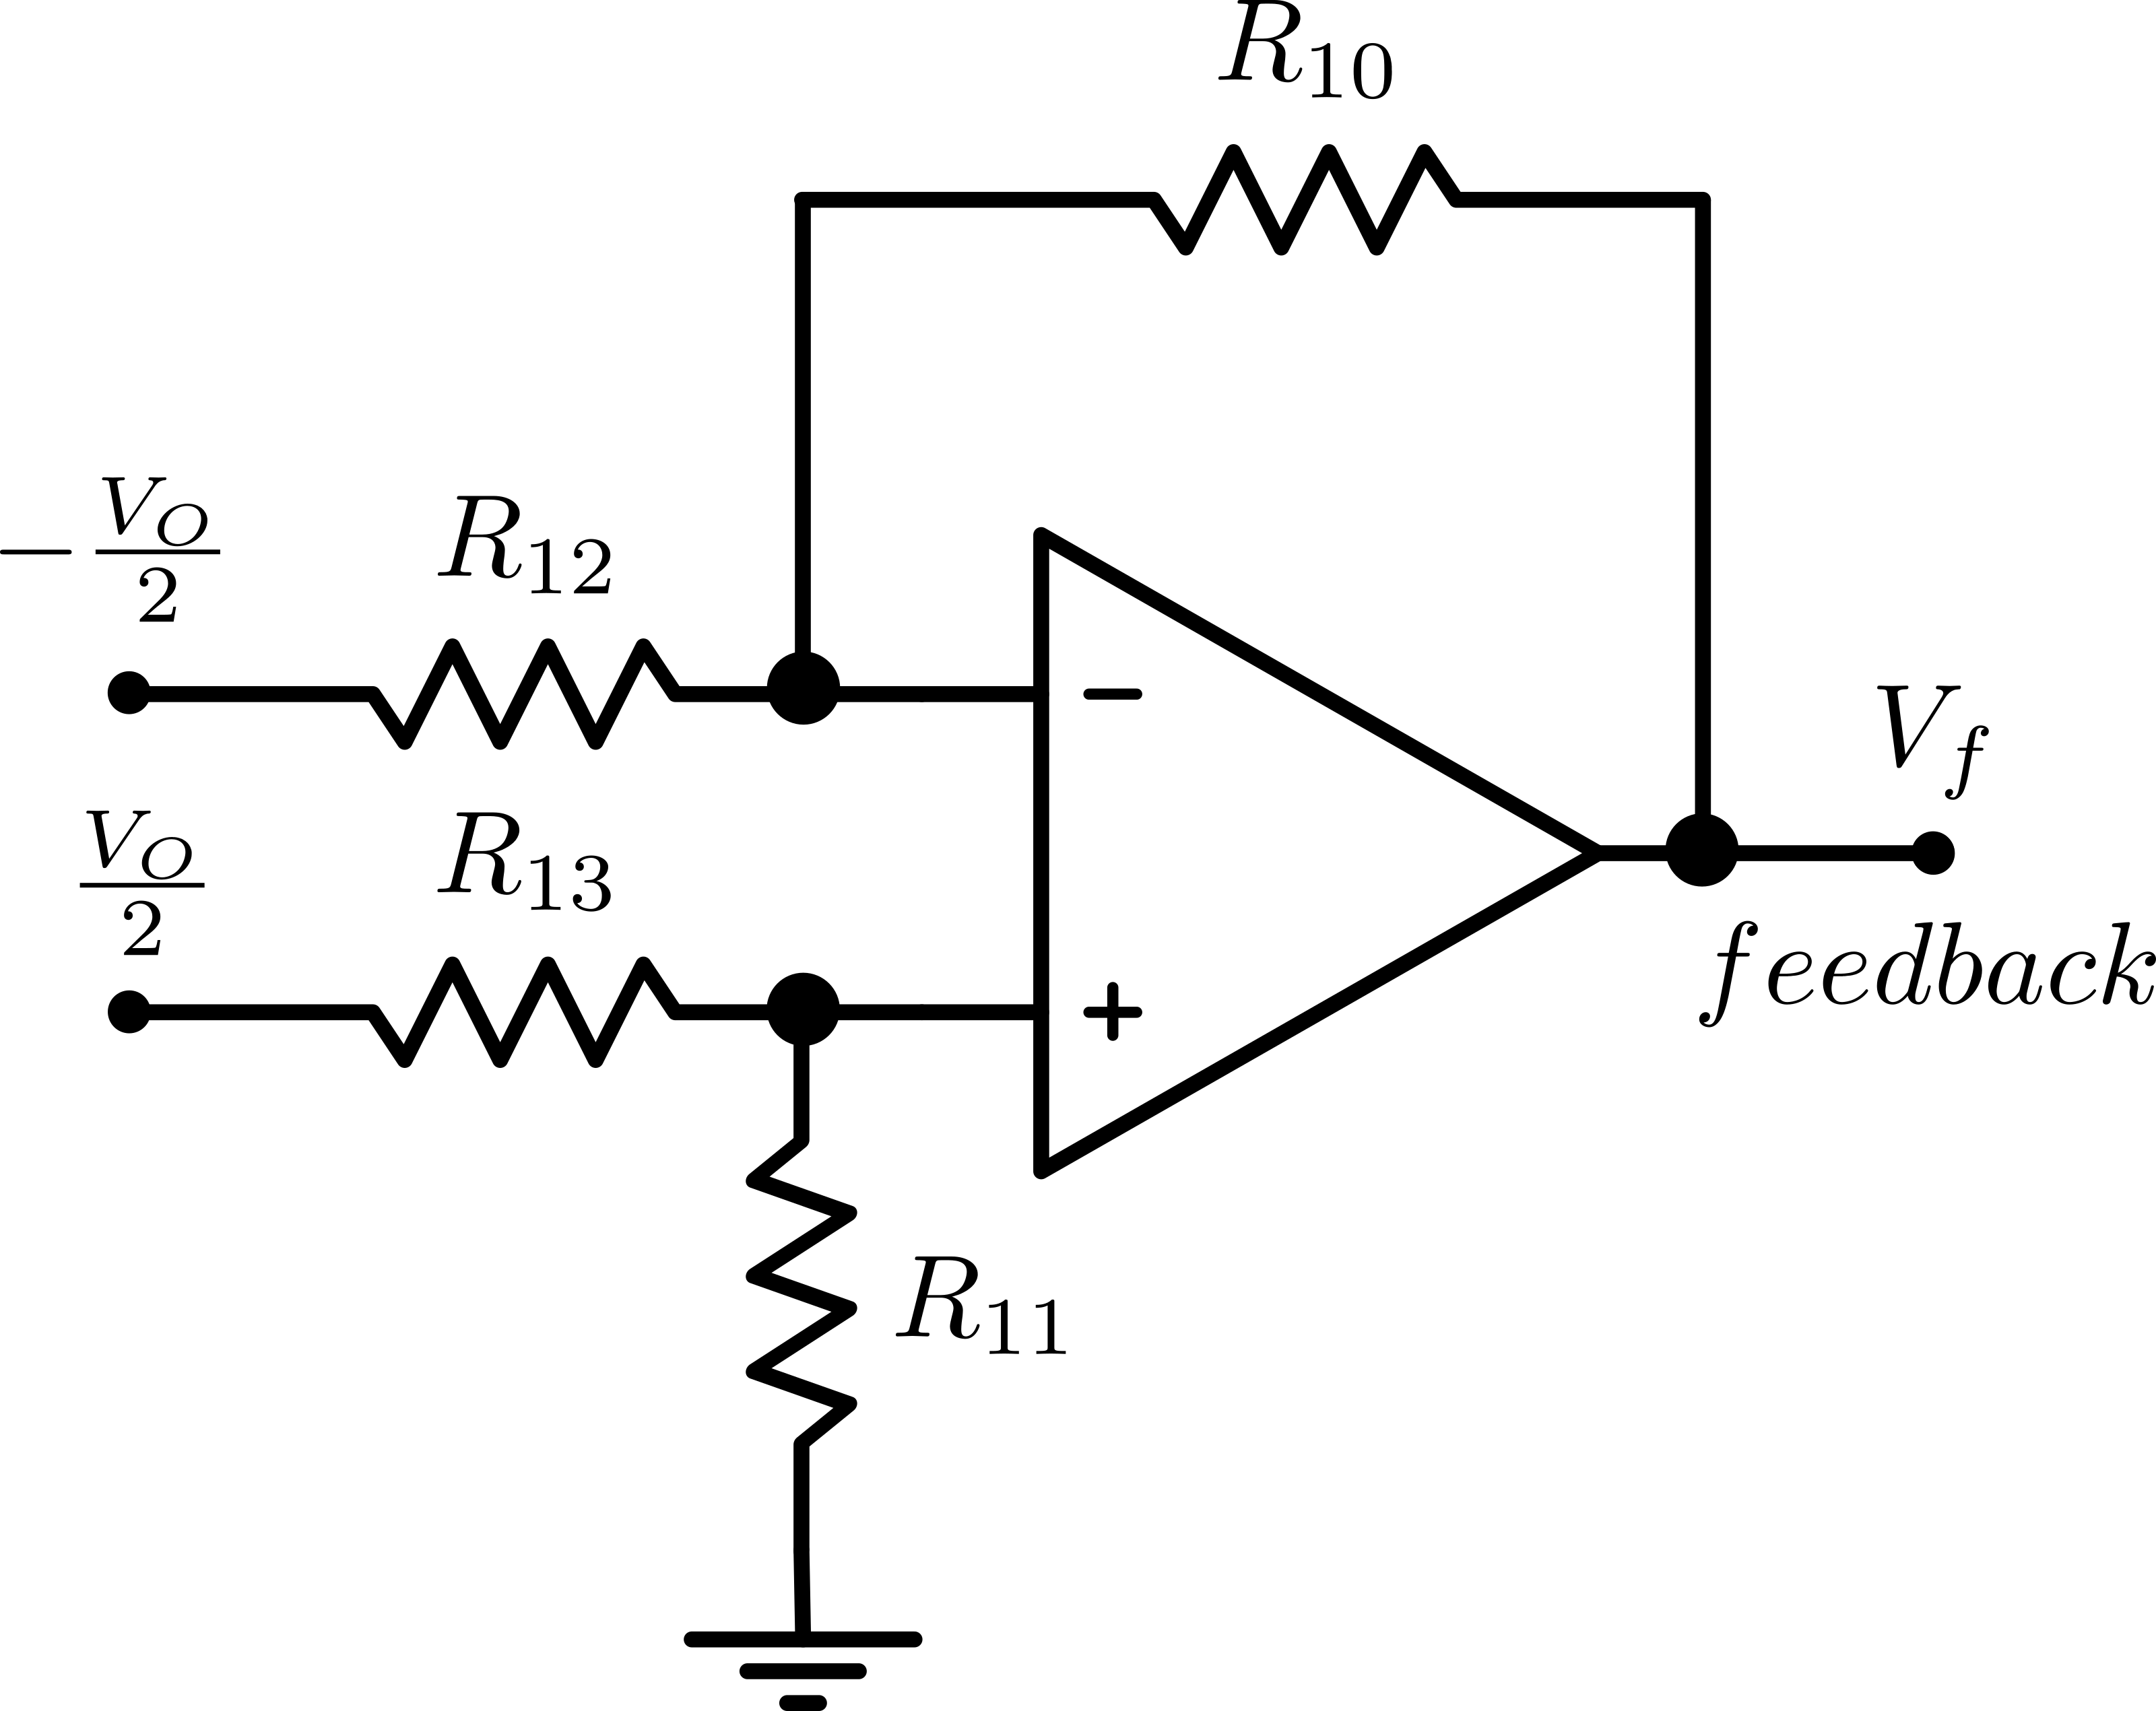
\includegraphics[scale=0.5]{Imagenes/Diferenciador.png}
\par\end{centering}
\caption{Diferenciador de señal de salida}
\end{figure}

Por superposición, la salida $V_f$ resulta:

\[
V_f = \frac{V_O}{2} \cdot \left( \frac{R_{11}}{R_{11} + R_{13}} \right) \cdot \left( 1 + \frac{R_{10}}{R_{12}} \right) + \left( -\frac{V_O}{2} \right) \cdot \left( -\frac{R_{10}}{R_{12}} \right)
\]

Si se toma $R_{10}(N) = R_{11}(N) = 1K\Omega$, y $R_{12}(N) = R_{13}(N) = (1K\Omega + 1K\Omega) = 2K\Omega$, queda:

\[
V_f = \frac{V_O}{2} \cdot \left( \frac{1}{3} \right) \cdot \left( \frac{3}{2} \right) + \frac{V_O}{2} \cdot \left( \frac{1}{2} \right) = \frac{V_O}{2}
\]

\subsubsection{Reestricción del ancho de banda}

Para limitar el ancho de banda del circuito, se agregan dos capacitores de compensación en el realimentador del circuito amplificador de tensión, como se muestra en la figura.

\begin{figure}[!ht]
\begin{centering}
\includegraphics[scale=0.5]{Imagenes/Opamp2ConCap.png}
\par\end{centering}
\caption{Amplificador de tensión e inversión de señal con límite de ancho de banda}
\end{figure}

Para las bajas frecuencias (en este caso menor a 20Hz), se busca que $C_2$ tenga una reactancia alta, comportándose como circuito abierto. En dicha situación, el amplificador queda con el formato de buffer, por lo que la continua pasa sin amplificarse. De esta forma, $C_2$ define la frecuencia de corte inferior.\par
Para altas frecuencias (en este caso, mayores a 20KHz), se busca que $C_1$ tengan una reactancia baja, de forma tal que la ganancia de la configuración de no inversor sea casi unitaria, para que mayores frecuencias no sean amplificadas. De esta forma, $C_1$ define la frecuencia de corte superior.\par
Para calcularlos, se tiene por un lado:

\[
f_{CI} = \frac{1}{2 \cdot \pi \cdot C_2 \cdot R_5}
\]
 
Dado que de los cálculos de ganancia anteriores se tiene $R_5$, se despeja el valor de $C_2$:

\[
C_2 = \frac{1}{2 \cdot \pi \cdot f_{CI} \cdot R_5} = 795nF \Longrightarrow C_2(N) = (470nF + 470nF) = 940nF
\]

Se redondea el valor teórico hacia arriba al normalizar, dado que la cota de 20Hz en audio es una cota inferior. Entonces, normalizando hacia arriba se tiene una $f_{CI}$ efectiva menor:

\[
f_{CI}^* = \frac{1}{2 \cdot \pi \cdot C_2(N) \cdot R_5(N)} = 16.9Hz
\]

De forma similar, para la otra cota:

\[
f_{CS} = \frac{1}{2 \cdot \pi \cdot C_1 \cdot R_6}
\]

De los cálculos de ganancia previos se tiene $R_6$, por lo que se despeja $C_1$:

\[
C_1 = \frac{1}{2 \cdot \pi \cdot f_{CS} \cdot R_6} = 41pF \Longrightarrow C_1(N) = 33pF
\]

Se redondea el valor teórico hacia abajo al normalizar, dado que la cota de 20KHz en audio es superior. Al normalizar hacia abajo, se tiene una $f_{CS}$ efectiva mayor:

\[
f_{CS} = \frac{1}{2 \cdot \pi \cdot C_1(N) \cdot R_6(N)} = 25.3KHz
\]

\subsection{Disipación de potencia}

Los transistores de potencia utilizados pueden soportar sin disipador una potencia de 2W (según hoja de datos ON Semiconductor). Para saber si requieren disipador, se calcula la potencia disipada en los mismos en el peor caso posible. Una forma simple de calcularla es obtener la potencia total entregada por las fuentes, y restar la potencia disipada por la carga $R_L$, ya que son las más significativas del circuito (junto con las potencias de los transistores).\par
Considerando la fuente de $+V_{CC}$, se tiene:

\[
P_{+V_{CC}} = V_{CC} \cdot \overline{I_{CC}}
\]
Dado que las fuentes entregan corriente en ambos semiciclos de la señal de entrada, la $I_{CC}$ tendrá formato de senoidal pero ambos semiciclos positivos. Se puede calcular la $\overline{I_{CC}}$ realizando la integral en un semiciclo y luego multiplicando el resultado por 2 debido a la simetría:

\[
\overline{I_{CC}} = 2 \cdot \frac{1}{T} \int_0^T \hat{I_O} \cdot sen(\omega t) \cdot dt = \frac{2}{\pi} \cdot \hat{I_O}
\]

Por lo que la potencia entregada por la fuente de $+V_{CC}$ resulta:

\[
P_{+V_{CC}} = V_{CC} \cdot \frac{2}{\pi} \cdot \hat{I_O} = V_{CC} \cdot \frac{2}{\pi} \cdot \frac{\hat{V_O}}{R_L}
\]

Entonces la potencia entregada por ambas fuentes resulta:

\[
P_{V_{CC}} = P_{+V_{CC}} + P_{-V_{CC}} = V_{CC} \cdot \frac{4}{\pi} \cdot \frac{\hat{V_O}}{R_L}
\]

Por lo tanto, para calcular la potencia disipada en los transistores, se le resta a esta última la potencia disipada por la carga, y se divide por 4 para obtener la potencia en cada transistor:

\[
P_{D_{Tx}} = \frac{1}{4} ( P_{V_{CC}} - P_O ) =  \frac{V_{CC}}{\pi} \cdot \frac{\hat{V_O}}{R_L} - \frac{\hat{V_O}^2}{8 \cdot R_L}
\]

Siendo 'x' cualquiera de los transistores $T_1$, $T_2$, $T_3$ y $T_4$. La expresión resultante es una parábola con concavidad hacia abajo, por lo que el máximo se halla en el vértice, que puede calcularse en forma sencilla derivando la expresión respecto a $\hat{V_O}$ e igualando a 0:

\[
\frac{dP_{D_{Tx}}}{d\hat{V_O}} = \frac{V_{CC}}{\pi \cdot R_L} - \frac{2 \cdot \hat{V_O}}{8 \cdot R_L} = 0
\]

\[
\left. \hat{V_O} \right|_{P_{D_{Tx}}\textrm{es máxima}} = \frac{4 \cdot V_{CC}}{\pi} = 19.09V < \hat{V_O}_{MAX}
\]

Reemplazando en la expresión de $P_{D_{Tx}}$ se halla entonces la potencia máxima disipada:

\[
\left. P_{D_{Tx}} \right|_{MAX} = \frac{2 \cdot V_{CC}^2}{\pi^2 \cdot R_L} = 5.7W
\]

Si el valor de $\hat{V_O}$ obtenido hubiera sido mayor al $\hat{V_O}_{MAX}$, el máximo estaría justamente en $\hat{V_O}_{MAX}$, ya que la $V_O$ no puede tomar un valor pico mayor a éste.\par
Dado que la potencia máxima obtenida resulta mayor a los 2W mencionados, se requiere añadirle un disipador a los transistores. Empleando el modelo conocido para relacionar la temperatura y potencia disipada mediante las resistencias térmicas, se tiene en este caso:

\[
P_{D_{Tx}} = \frac{T_J - T_A}{\theta_{JC} + \theta_{CD} + \theta_{DA}}
\]

De la hoja de datos utilizada (ON Semiconductor):

\[
T_J = 150^{\circ}C \hspace{2cm} R_{\theta_{JC}} = 1.95 \left(\frac{^{\circ}C}{W}\right)
\] 
 
\[
\left\lbrace
\begin{array}{l}
R_{\theta_{JC}}: \textrm{Resistencia t\'ermica entre juntura y carcasa del transistor} \\
R_{\theta_{CD}}: \textrm{Resistencia t\'ermica entre carcasa y el disipador} \\
R_{\theta_{DA}}: \textrm{Resistencia t\'ermica entre disipador y ambiente}
\end{array}
\right.
\] 

Dado que se colocará el disipador directamente sobre el transistor mediante pasta térmica, se puede considerar una $R_{\theta_{CD}} \approx 1 \left(\frac{^{\circ}C}{W}\right)$, y se considera como temperatura ambiente $T_A = 30^{\circ}C$. Se despeja entonces el valor de la $R_{\theta_{DA}}$:

\[
R_{\theta_{DA}} = \frac{T_J - T_A}{P_{D_{Tx}}} - R_{\theta_{JC}} - R_{\theta_{CD}} = 18 \left(\frac{^{\circ}C}{W}\right)
\]

De los disipadores que se disponían, se utilizó el ZD35 (modelo de 5cm de altura), que cumple con una $R_{\theta_{DA}} = 10 \left(\frac{^{\circ}C}{W}\right)$, que se muestra en la siguiente figura.

\begin{figure}[!ht]
\begin{centering}
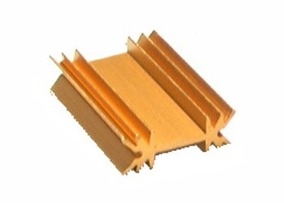
\includegraphics[scale=0.5]{Imagenes/ZD35.jpg}
\par\end{centering}
\caption{Disipador ZD35 - Modelo de alto 5cm}
\end{figure}

\newpage

\section{Implementación - Análisis de parámetros característicos}

\subsection{Rendimiento}

El rendimiento del amplificador se define como: 

\[
\eta(\%) = \frac{P_O}{P_{V_{CC}}}
\]

Si se reemplazan las expresiones de potencia total entregada por las fuentes y la potencia de salida, resulta:

\[
\eta(\%) = \frac{\hat{V_O} \cdot \pi}{8 \cdot V_{CC}} 
\]

Se obtiene entonces el rendimiento máximo con la $\hat{V_O}_{MAX}$:

\[
\eta(\%) = 52.3\%
\]

\subsection{Respuesta en frecuencia}

\subsubsection{Ganancia de lazo - Compensación}

El circuito propuesto tal como está planteado, si se simula la ganancia de lazo (mediante el script provisto por la cátedra), puede observarse que cuando la magnitud cruza los $0dB$, el margen de fase es negativo, surgiendo oscilaciones en torno a la frecuencia de 1MHz. El diagrama se muestra en la figura siguiente.

\begin{figure}[!ht]
\begin{centering}
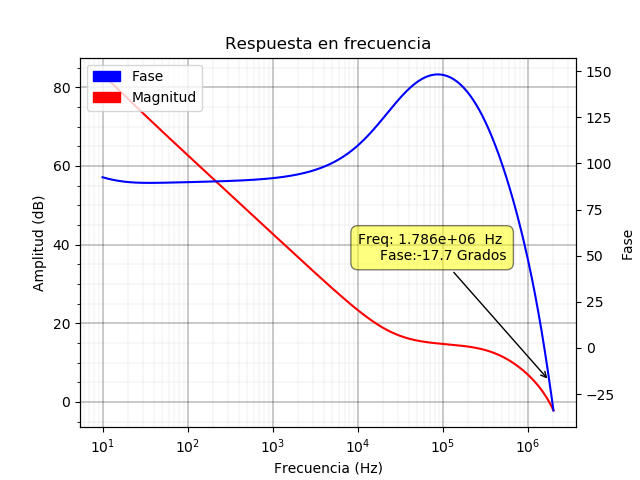
\includegraphics[scale=0.45]{Imagenes/LazoSinCompenzar.png}
\par\end{centering}
\caption{Ganancia de lazo (módulo y fase) sin compensar - Gráfico realizado en Python}
\end{figure}

Para mejorar el margen de fase para evitar la oscilación, se colocó un capacitor en la resistencia de realimentación del amplificador operacional que realiza la diferenciación de la señal de salida (es la $R_8$). Su valor se determinó mediante simulaciones sucesivas (llegando a un valor final de $C_{COMP} = 1nF$) hasta obtener un margen de fase holgado, logrando un valor de aproximadamente $70^{\circ}$, como se muestra en la siguiente figura.

\begin{figure}[!ht]
\begin{centering}
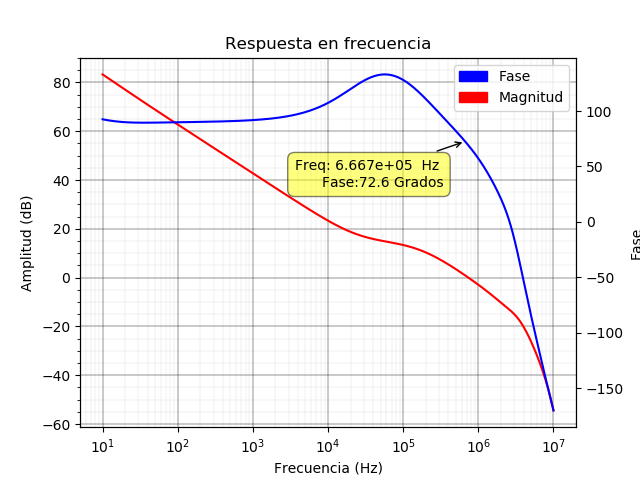
\includegraphics[scale=0.45]{Imagenes/LazoCompenzar.png}
\par\end{centering}
\caption{Ganancia de lazo (módulo y fase) compensada - Gráfico realizado en Python}
\end{figure}

\subsection{Impedancia de entrada}

Dado que a la entrada desde el generador se ve la entrada del amplificador operacional en configuración de no inversor, la impedancia vista es la de entrada del operacional, multiplicada por el factor (1+|T|) dado que el lazo de realimentación suma tensión. La impedancia de entrada del TL084 es del orden de $10^{12}\Omega$, por lo que multiplicada por Es decir que (1+|T|) resulta prácticamente infinita. Para cumplir con un poco de margen con la característica pedida de $Z_{IN} = 50K\Omega$, se coloca en paralelo a la entrada del operacional una resistencia de $56K\Omega$. Al tener una impedancia muy grande en paralelo a la de $56K\Omega$, la vista por el generador a la entrada resulta prácticamente $56K\Omega$.

\subsection{Impedancia de salida}

%CREO QUE DE BAJA

\subsection{Distorsión armónica}

\end{document}
